\documentclass[letterpaper,12pt]{article}
\usepackage{fullpage}
\usepackage{fancyvrb,fancyhdr}
\usepackage{amsfonts}
\usepackage{array}
\usepackage{multirow}
\usepackage{amsmath, amssymb, amsthm}
\usepackage{graphicx,longtable, booktabs}
\usepackage[flushleft]{threeparttable}
\usepackage[footnotesize,center]{subfigure}
\usepackage{enumerate}
\usepackage{lastpage}
\usepackage{url}
\usepackage{mathrsfs}
\usepackage{cancel}
\usepackage{cite}
\usepackage{soul}
\usepackage{MnSymbol}
% Pseudo Code
\usepackage{algorithm}
\usepackage{algorithmic}
% Comments are in red
\usepackage{color}

\oddsidemargin 0in \evensidemargin 0in
\topmargin -0.5in \headheight 0.25in \headsep 0.25in
\textwidth 6.5in \textheight 9in %\marginparsep 0pt \marginparwidth 0pt
\parskip 0ex \parindent 10pt \footskip 20pt

\newfont{\bssten}{cmssbx10}
\newfont{\bssnine}{cmssbx10 scaled 900}
\newfont{\bssdoz}{cmssbx10 scaled 1200}

\pagestyle{fancy}
\fancyhead[LO]{\bssnine ConvNN used in DR classification }
% \fancyhead[R]{} \fancyhead[LO]{}
\fancyhead[RO]{\bssnine \thepage/\pageref{LastPage}}
%\fancyhead[RO]{\thepage}
\lfoot{} \cfoot{} \rfoot{}

%\usepackage[pdftex]{hyperref}

\def\t#1{{\tt #1}}
\newfont{\sserifn}{cmssbx10 at 11pt}
\newfont{\sserifo}{cmssbx10 at 12pt}

% Defining new \vect{} command to use a bold letter as a vector
\newcommand{\vect}[1]{\mathbf{#1}}
\newcommand{\erfc}{\mathrm{erfc}}
\newcommand{\figref}[1]{Figure~\ref{#1}}
\newcommand{\tableref}[1]{Table~\ref{#1}}
\newcommand{\eqsref}[1]{Eq.~\ref{#1}}
\newcommand{\algref}[1]{Algorithm~\ref{#1}}

%opening                    

\usepackage[para,multiple]{footmisc}
\newcommand{\jose}[1]{\comment{red}{#1}}
\newcommand{\imagej}{ImageJ }

\title{Convolution Neural Network Approach to Diagnosing Diabetic Retinopathy}
\author{Jos\'e Solomon \thanks{jose.e.solomon@gmail.com} } 

\date{}
\begin{document}

\maketitle
\begin{abstract}
This is the first draft of the report for my project on diabetic retinopathy diagnosis using convolution neural networks (ConvNN). It is derived from the Kaggle Diabetic Retinopathy Challenge \cite{kaggle} aimed at creating a robust algorithm to automate the process of classifying the level of diabetic retinopathy found in retinal scans. The purpose of this initial draft is primarily to describe how ConvNN work, and the inter-dependencies  of its various functional elements. 
\end{abstract}
\tableofcontents

\section{Introduction}

There are two key facets to the project: first is the concept of the diabetic retinopathy and its diagnosis; the second is ConvNNs and their general functioning principles as applied to digital imaging processing and categorization. We begin with a cursory description of the former, and then focus the bulk of the theoretical discussion on the latter.

\section{Diabetic Retinopathy}

Diabetic retinopathy (DR) is a disease that generally afflicts those who have dealt with diabetes for a period of 5 years or more \cite{nih}. It is defined specifically as the deterioration of blood vessels found or that lead to the retina of the human eye, as illustrated in \figref{eye} below.

\begin{figure}[htbp]
\begin{center}
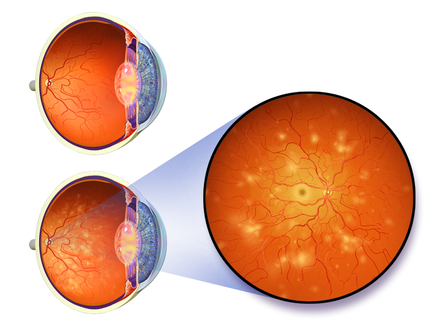
\includegraphics[scale=0.6]{images/illustration.png}
\caption{Diabetic retinopathy in comparison to a normal eye \cite{wiki}, (shown at the top left)}
\label{eye}
\end{center}
\end{figure}

The primary cause of DR is a byproduct of the condition of diabetes, where finer blood vessels in the human body tend to form abnormal branching structures and begin to exhibit thinning walls. This leads to deteriorated blood supply to the effected areas and eventually to hemorrhaging. In terms of the retina, this leads to blind spots forming in the field of vision of the afflicted individual. 

To diagnose the condition, a retinal scan of the eye is taken and a classification is assigned based on a combination of the following features: the number of abnormal vein branching seen, the general wall thickness of the blood vessels, and the number of blood stains observed due to hemorrhaging. DR is categorized on a scale from 0 to 4, and examples of level 0 and level 4 DR are shown in \figref{marking_image}. It should be noted that this method of categorizing DR is not fundamentally rigorous in nature and is more of a qualitative scale. 

\begin{figure}[htbp]
\begin{center}
 \subfigure[Level 0 DR]{\label{reference}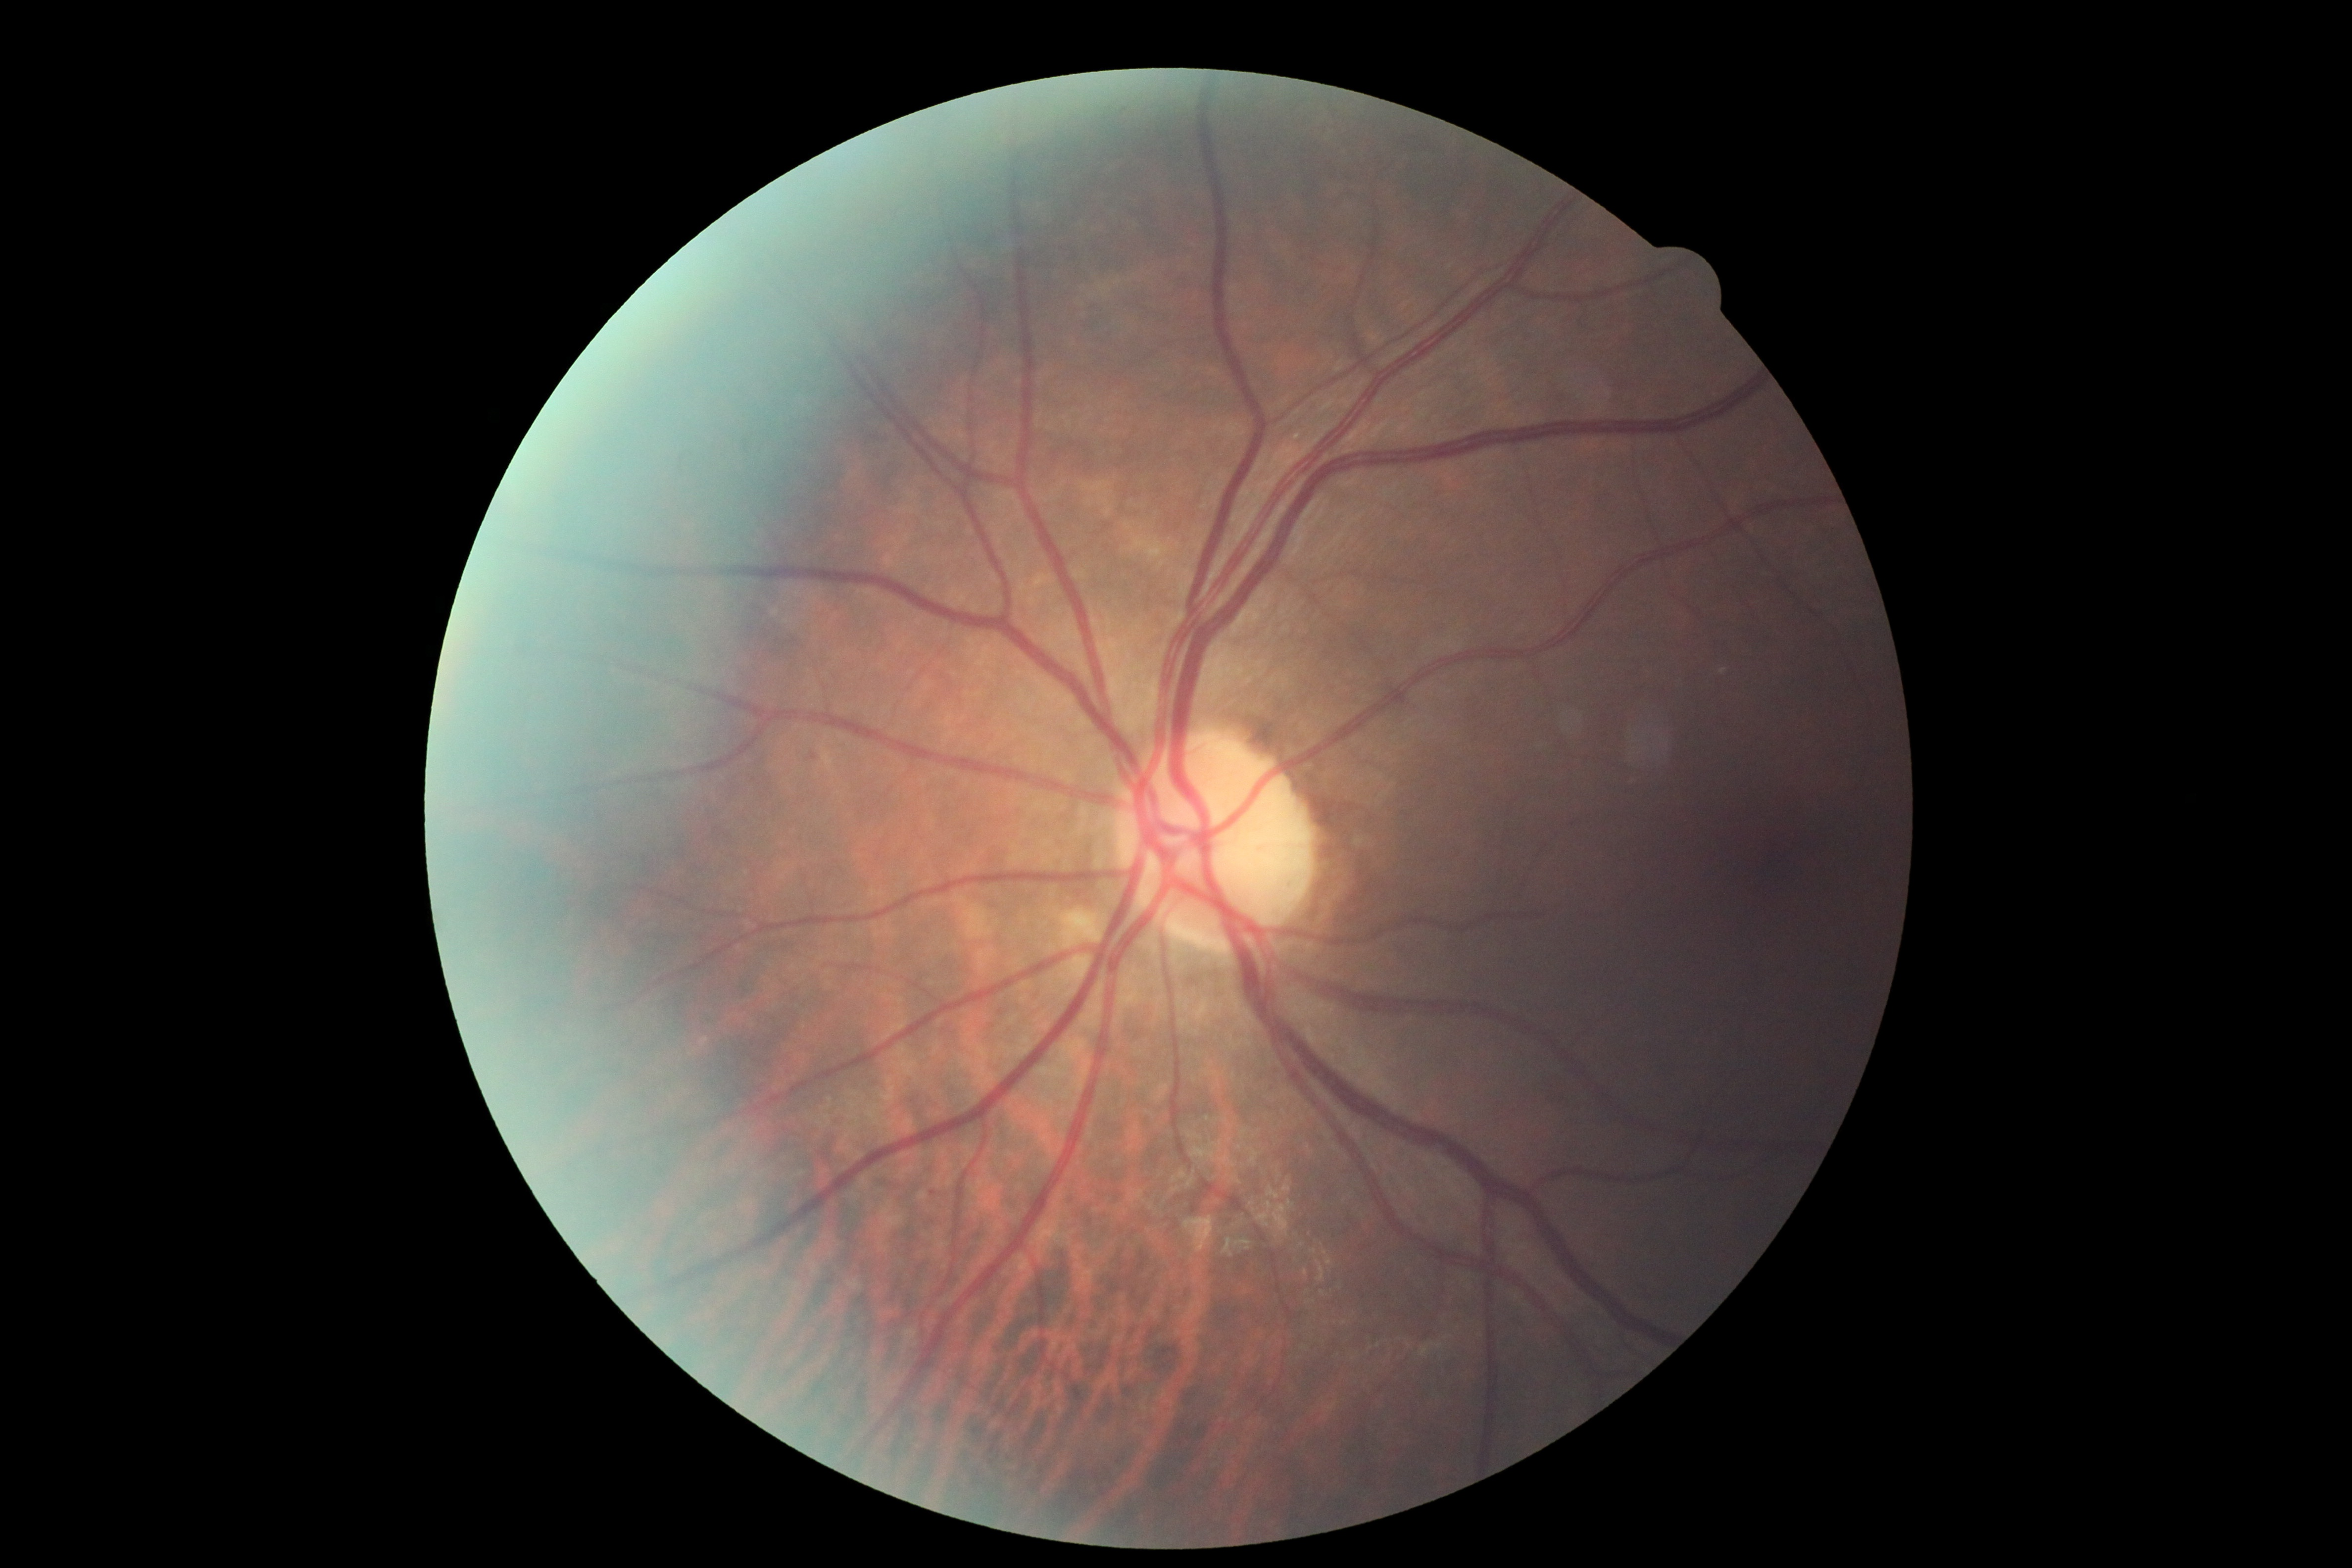
\includegraphics[scale=0.035]{images/0_Level_Example.jpeg}}
  \ \ \ \ 
\subfigure[Level 4 DR]{\label{new}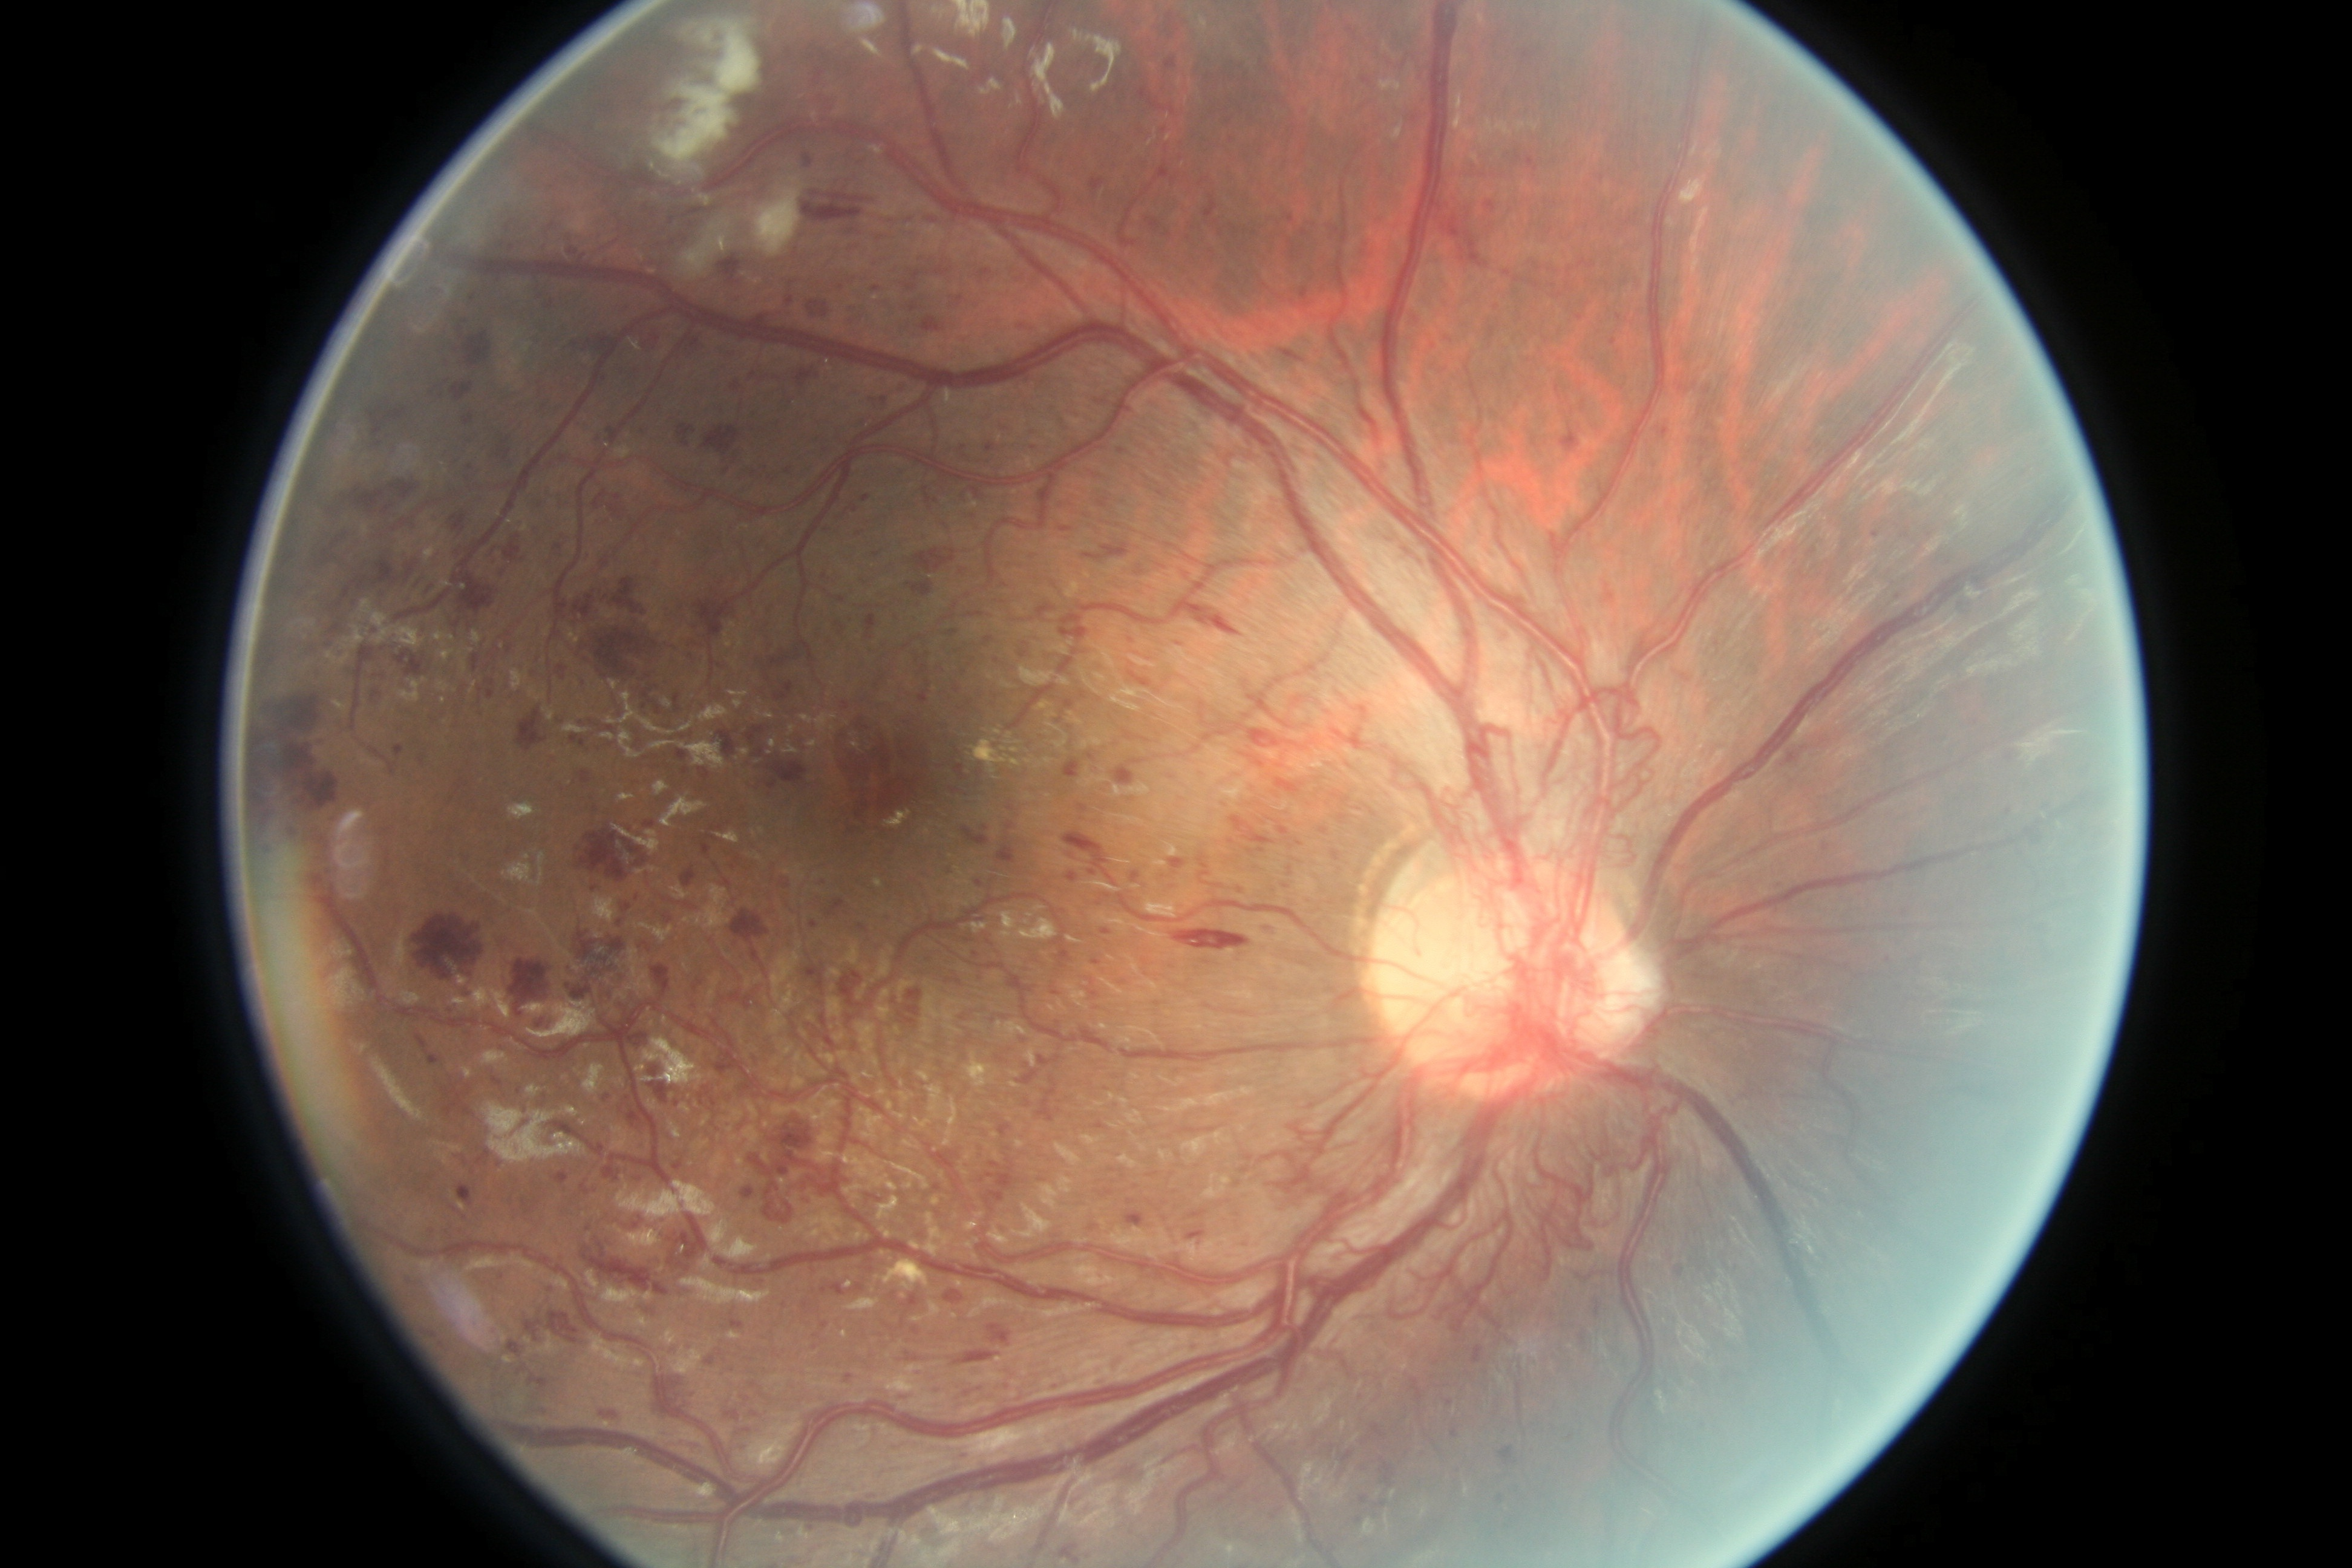
\includegraphics[scale=0.0425]{images/4_Level_Example.jpeg}}
\caption{Examples of level 0 and level 4 DR}
\label{marking_image}
\end{center}
\end{figure}

\subsection{The Kaggle Grand Challenge}

Kaggle has presented the automated DR diagnosis as an open grand challenge. In doing so, Kaggle provided more than 35 gigabytes of retinal scan data, (over 35,000 images), where each image is roughly 1.5 megabytes in size. To aid in download and processing of the data set, Kaggle divided the image set into a training group and a testing group, and then subsequently divided each group into smaller subsets to facilitate file transfer. All the results presented here and in subsequent discussions are based on the first training set of images.

It is noted that the aim of the current work is to understand ConvNN from a fundamental perspective, and not to actually create a competitive solution for the grand challenge. Due to the size of the reference data set, and the limitations imposed by Python in terms of loading elements into shared memory, it would be very difficult to create a code base that could compete directly with other implementations in CuDa, (a GPU-level system language), which is the de facto favorite language for image processing.	

\section{Convolution Neural Networks}

ConvNN is a powerful machine learning technique that falls under the general premise of deep learning. There are number of flavors of ConvNN, but the specific implementation presented here is one derived from of the first concrete examples of the technique, the LeNet-5 \cite{LeNet}, which is especially adept at processing digital imaging.

The LeNet-5 consists of 3 primary component layers: the convolution layer, the pooling layer, and the conventional fully connected layer \cite{deep}. 

\subsection{The Convolution Layer}

The convolution layer is the work horse of the ConvNN, and it is what makes it such an indispensable tool for image processing. Mathematically, the concept of convolution is somewhat straightforward, and plays a key role in spectral methods/Fourier transform treatments. In terms of digital imaging, convolution can be expressed as \cite{deep} the product of the pixel intensity of a given image with that of a kernel, and is stated as
\begin{equation}
H[m,n] * G[m,n] \, = \, \sum_{u=- \infty}^{\infty} \sum_{u=- \infty}^{\infty} H[u,v] G[m-u, n-v]
\end{equation}

This may seem somewhat complex at first, but consider that a digital image is an array of pixels, each with an intensity that ranges from 0 up to a given bit depth, (e.g. 255 for 8-bit images), than we can see that an image can be translated as matrix, where each element is a given pixel's image intensity. The concept is illustrated in \figref{lena}.
\begin{figure}[htbp]
\begin{center}
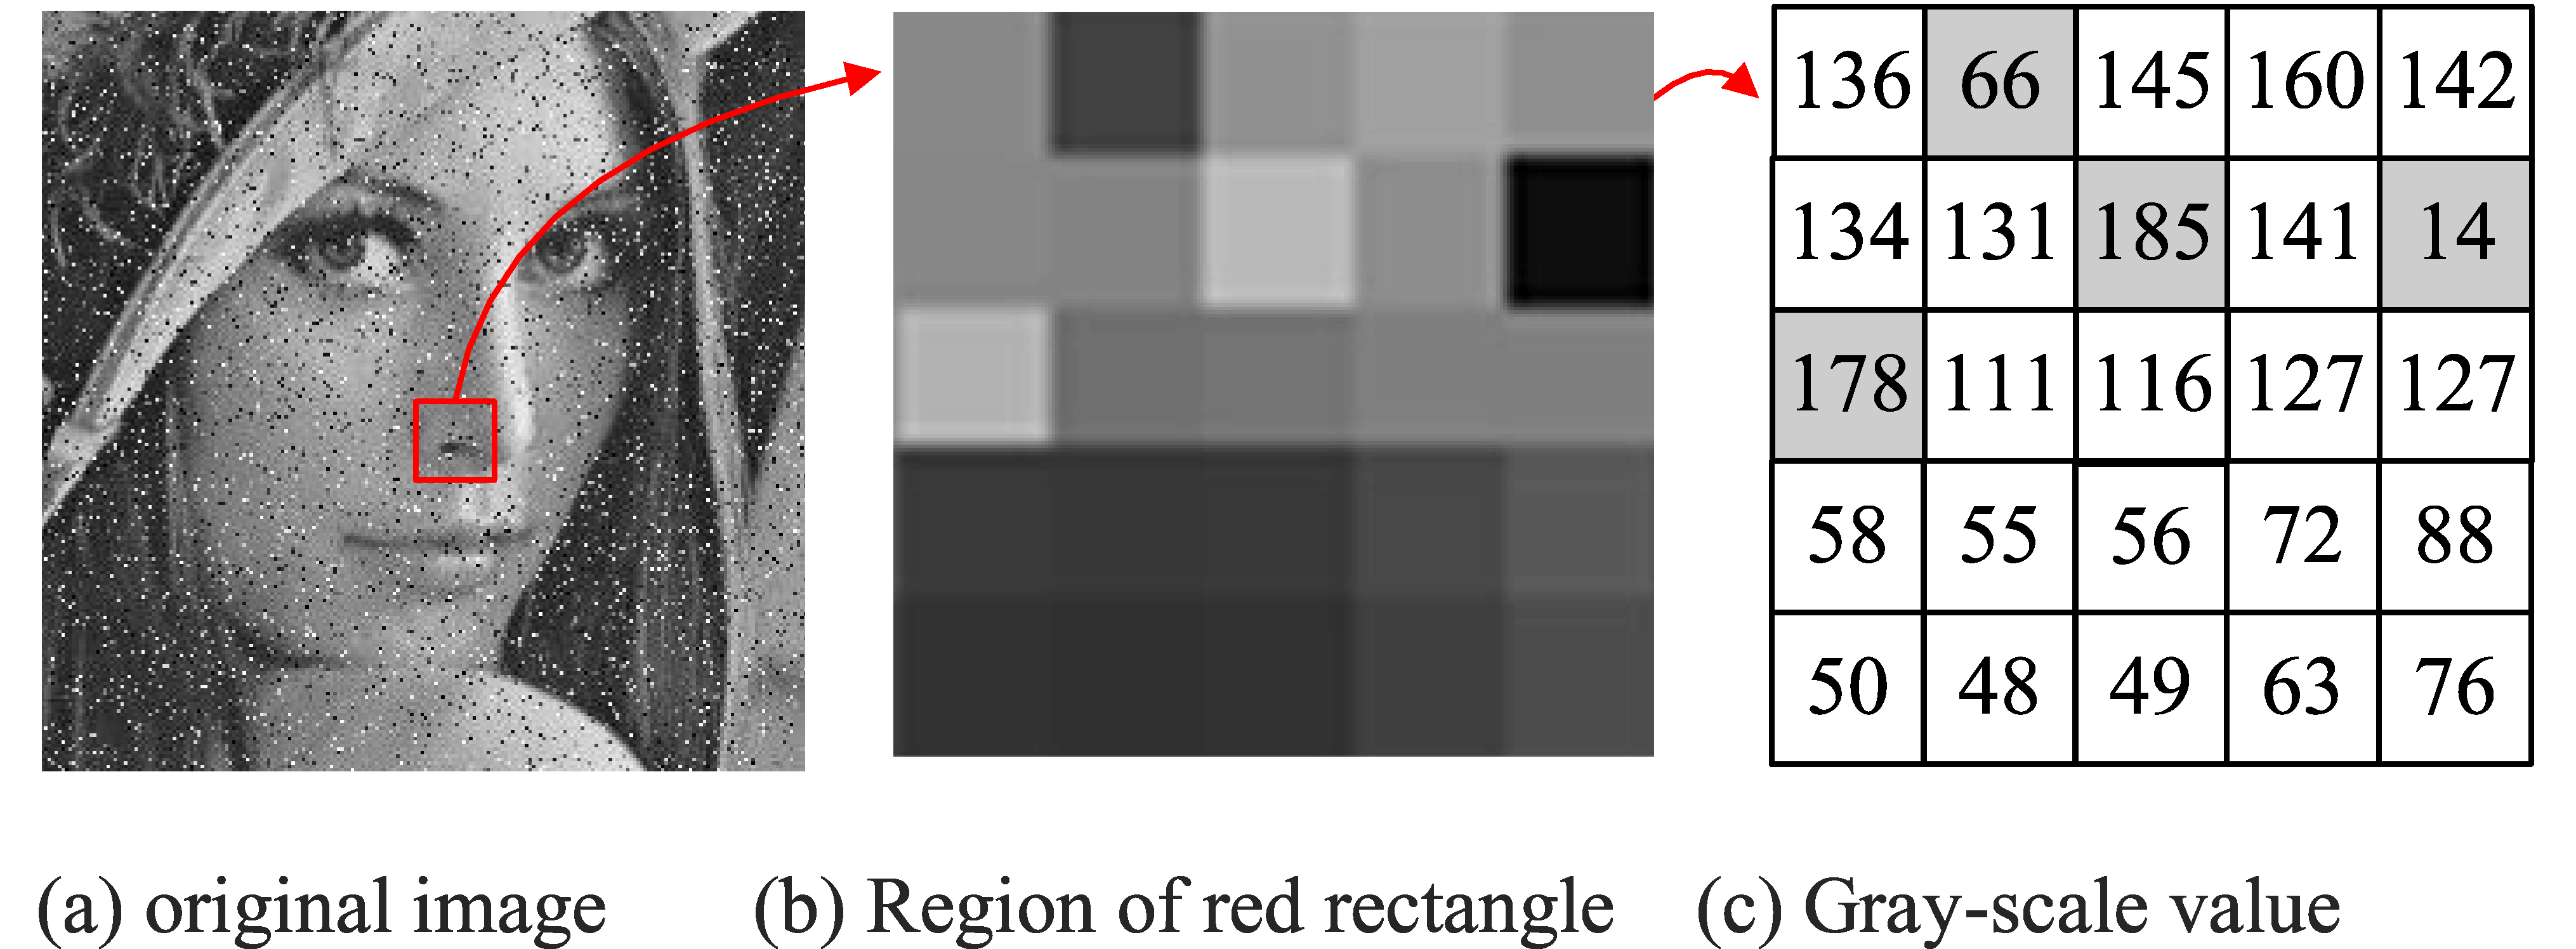
\includegraphics[scale=0.1]{images/lena.png}
\caption{Digital image as a matrix \cite{lena}}
\label{lena}
\end{center}
\end{figure}

With this concept in place, a kernel is itself a matrix of a prescribed dimension, smaller than that of the original image,  an example of which would be
\begin{equation}
H_{3 \times 3}^L \, = 
\begin{bmatrix}
  0 & 1  & 0 \\
  1 & -4 & 1 \\
  0 & 1  & 0
\end{bmatrix}
\label{lap_3x3}
\end{equation}

This matrix is applied, via convolution, across the matrix of the image to create a filtered image which, depending on the \textit{stride}, (i.e. number of times the kernel is applied across the original image), downsizes the original image into smaller matrix which is representative of the dot product between the original image and kernel.  The full convolution concept is illustrated in \figref{conv}. 

\begin{figure}[htbp]
\begin{center}
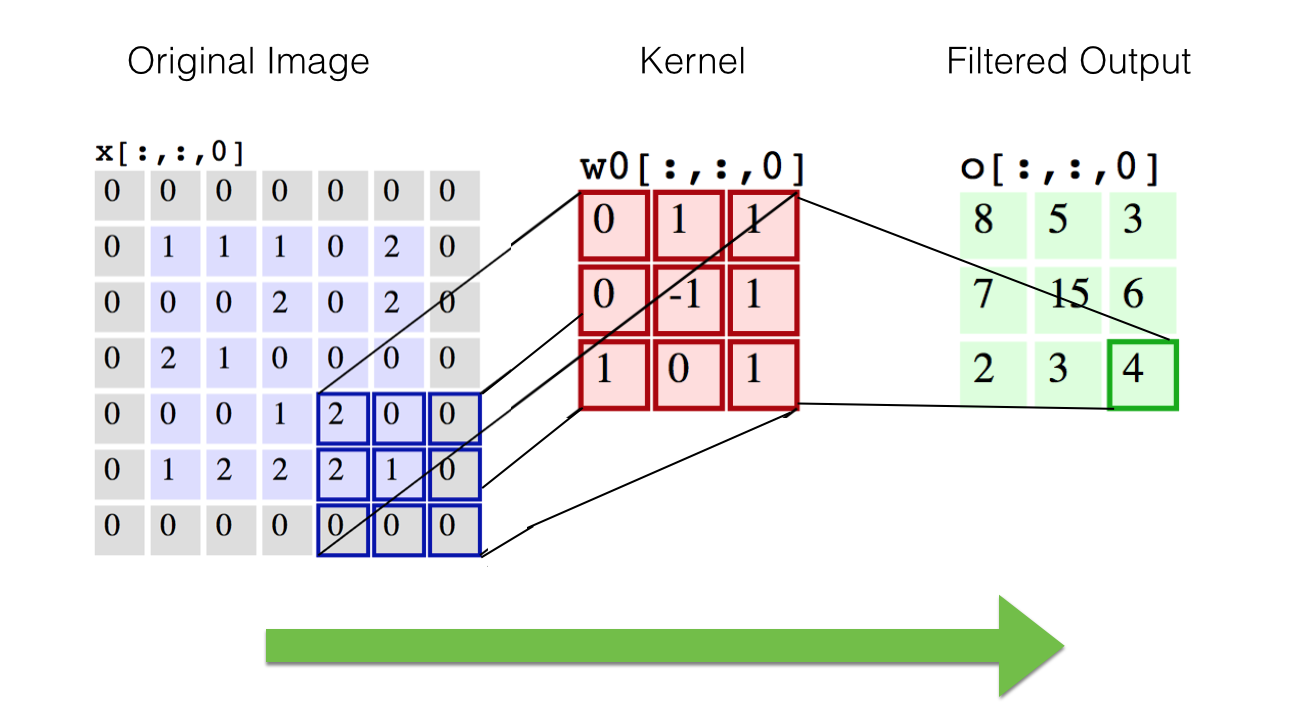
\includegraphics[scale=0.7]{images/convolution.png}
\caption{Convolution concept \cite{cs231}}
\label{conv}
\end{center}
\end{figure}

\subsection{The Pooling Layer}

In order to reduce the computational expenditure of the ConvNN algorithm, a pooling module is often used to reduce the required number of weights for a subsequent fully connected neural network layer.  

Usually the form of the pooling is \textit{max pooling}, where  a specific number of elements of the convoluted image are defined as common-pool members, (as illustrated in \figref{maxPool}), and only the pool member with the maximum value is carried forward in the network. The size of a pool is usually, but not required to be, the same size as the kernel applied during convolution. By focusing on the maximum value of a convolution, the network is becoming more sensitive to those image features which are more dominant in the total feature set.

\begin{figure}[htbp]
\begin{center}
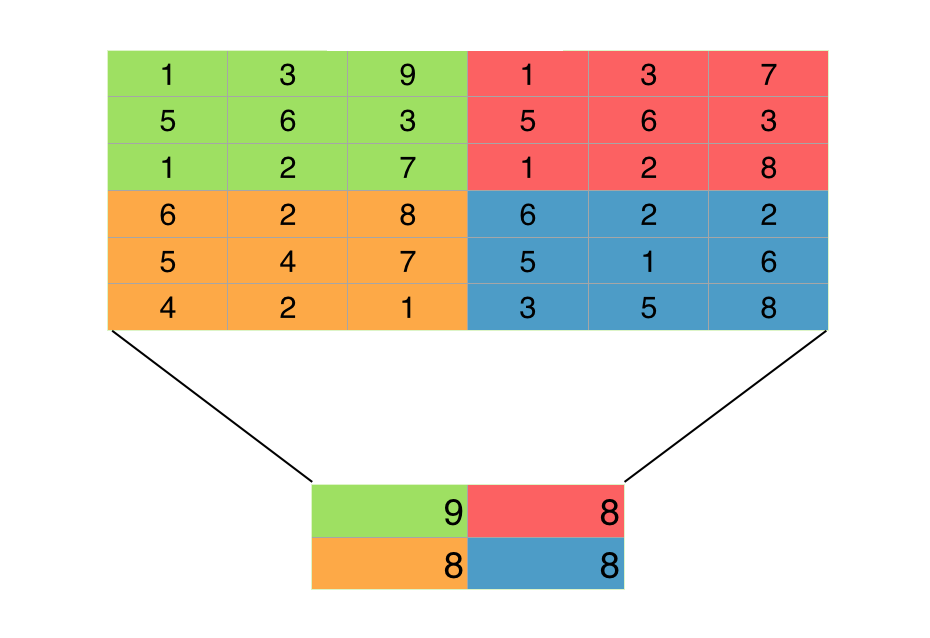
\includegraphics[scale=0.6]{images/maxpool.png}
\caption{Max-pooling: the largest value of each sub-cell is fed forward}
\label{maxPool}
\end{center}
\end{figure}

It is noted that a ConvNN often uses a series of convolution and pooling layers to continuously reduce the computational load of the final layer, or layers, of fully connected NN, which is normally the most computational expensive facet of the ConvNN pipeline. 

\subsection{The Fully Connected NN Layer}

The fully connected NN layer is actually a \textit{conventional} neural network, which is comprised of a series of nodes that are interconnected via a series of weights and bias units. Let's begin with the illustration shown in \figref{ann}.

\begin{figure}[htbp]
\begin{center}
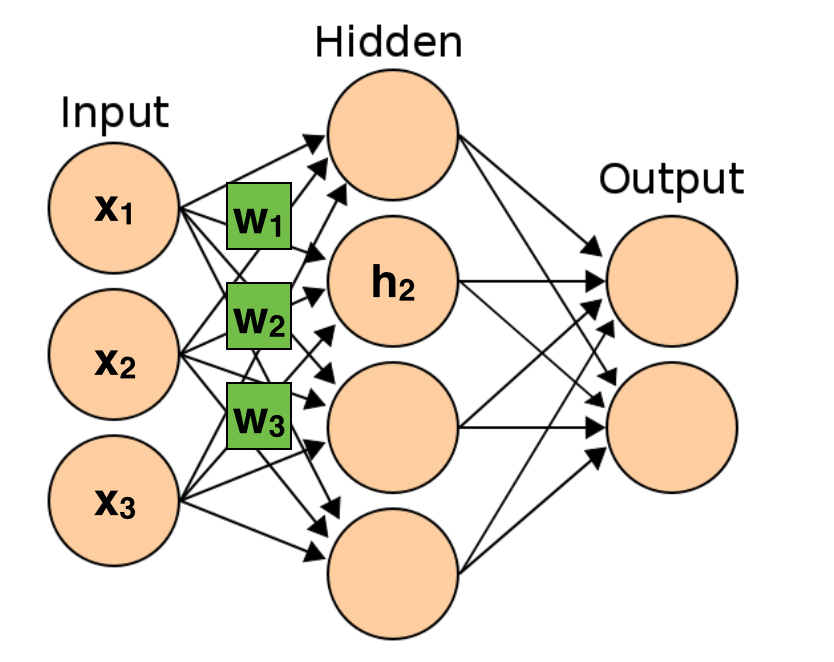
\includegraphics[scale=0.5]{images/nn_edit.png}
\caption{A fully connected neural network \cite{ann}}
\label{ann}
\end{center}
\end{figure}

As can be seen from the figure, each node is connected to the series of nodes in the layer directly downstream of it. The nodes downstream are in turn connected to each node in the layer upstream of them, as well as each node in the layer downstream of them. The result is a series of nodes that are \textit{fully} interconnected.

Let's say that for each input connection of a given node, there is an associated weight $w_i$. Given that there is $N$ number of nodes in the upstream layer, the input to the downstream node can be seen as 
\begin{equation}
f(\vec{w}^T\vec{x}) \, = f(w_0 \cdot x_0 + w_1 \cdot x_1 + \cdots + w_N \cdot x_N)
\end{equation}

We note that the dot product $\vec{w}^T\vec{x}$ is the input to a function, known as the activation function, which in turn is the input value of the downstream node. There are a variety of activation functions that can and have been used in NN. One of the most popular, and the one which is used here, is the \textit{tanh} activation function, which is defined as
\begin{equation}
f_{\text{tanh}}(a) \, = \frac{e^a-e^{-a}}{e^a+e^{-a}}
\end{equation}
which has an activation profile shown in \figref{tanh} As can be seen, the function has asymptotes  at 1 and -1 and exhibits positive values in $y$ for positive values of $x$. Another common activation function is the sigmoid activation function, which has a similar profile as \textit{tanh} and has the functional form
\begin{equation}
f_{sigmoid}(a) \, = \frac{1}{1-e^{-a}}
\end{equation}
As shown in \figref{sig}, the sigmoid activation function has asymptotes at 1 and 0, and is centered at the origin in $x$ and at 0.5 in $y$. 

\begin{figure}[htbp]
\begin{center}
 \subfigure[Tanh Function]{\label{tanh}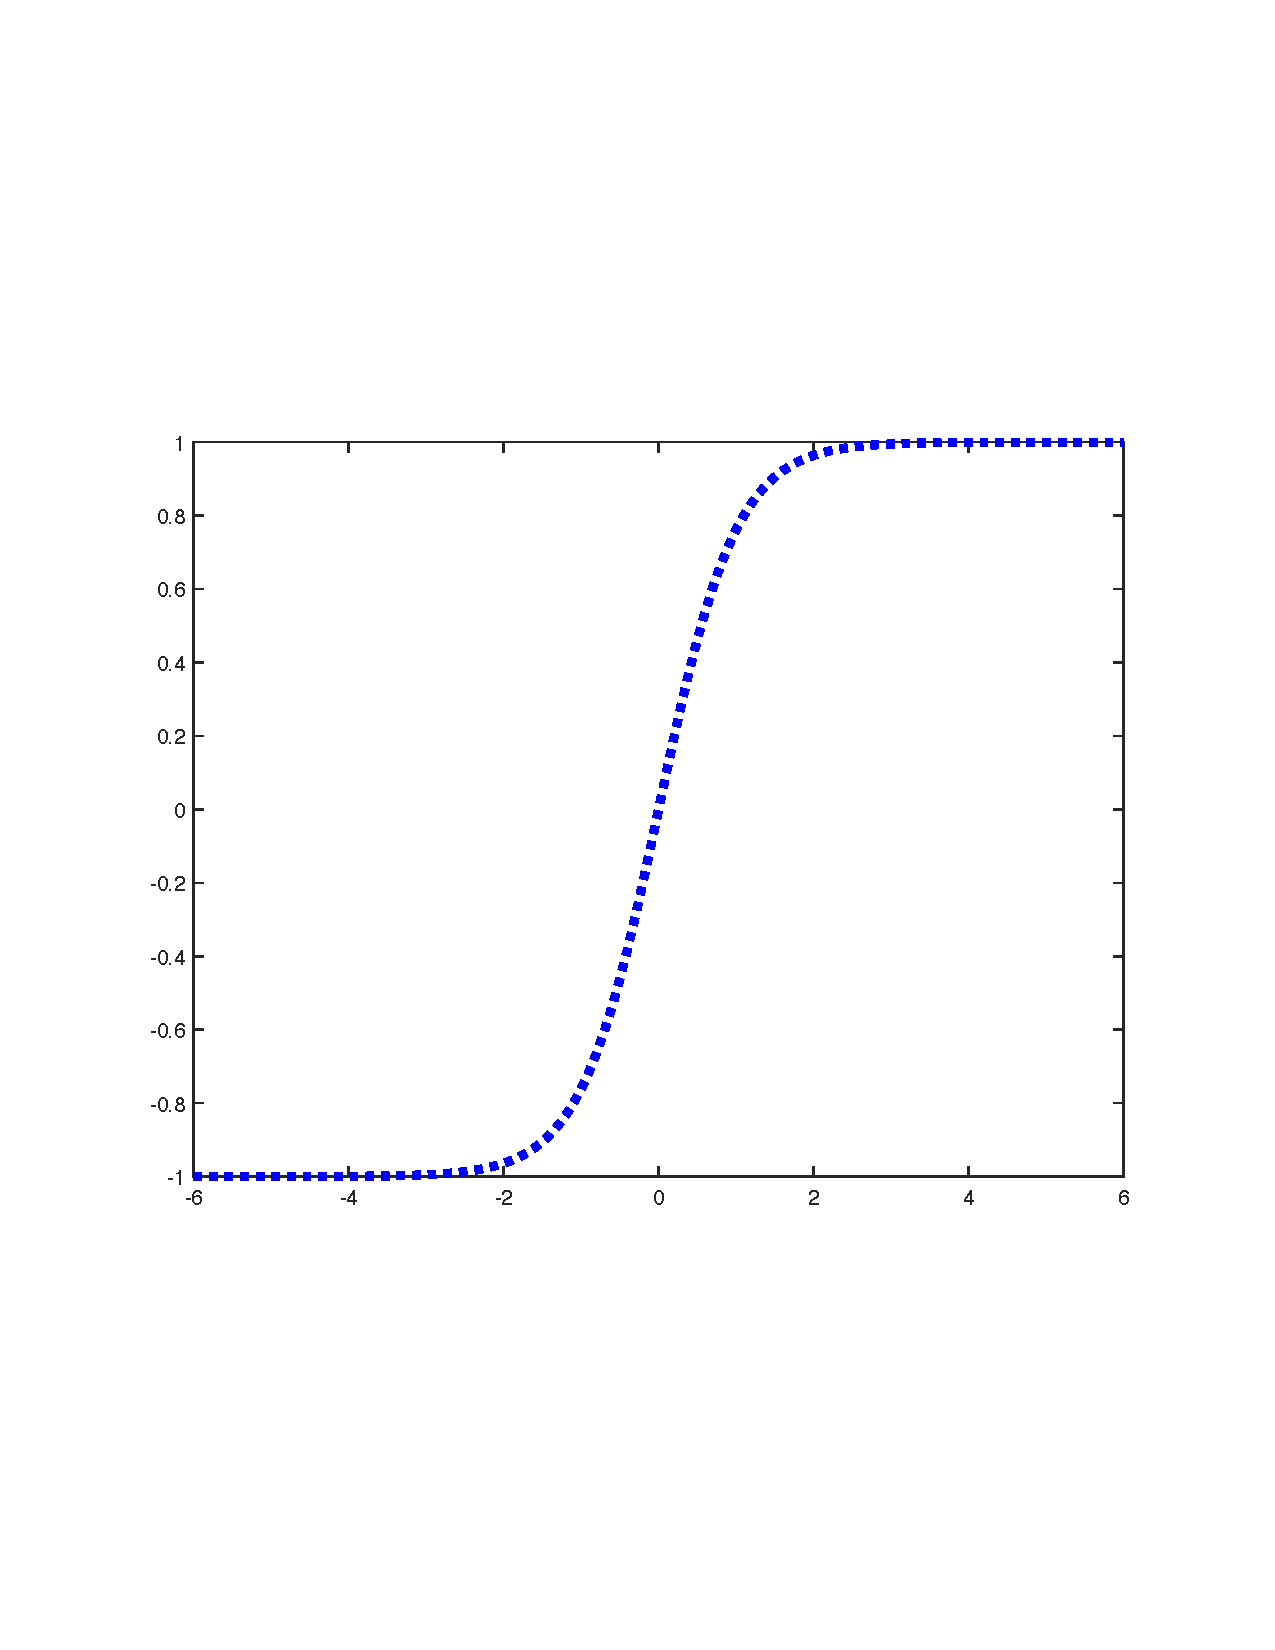
\includegraphics[scale=0.45]{images/TanhFunction.pdf}}
  \ \ \ \ 
\subfigure[Sigmoid Function]{\label{sig}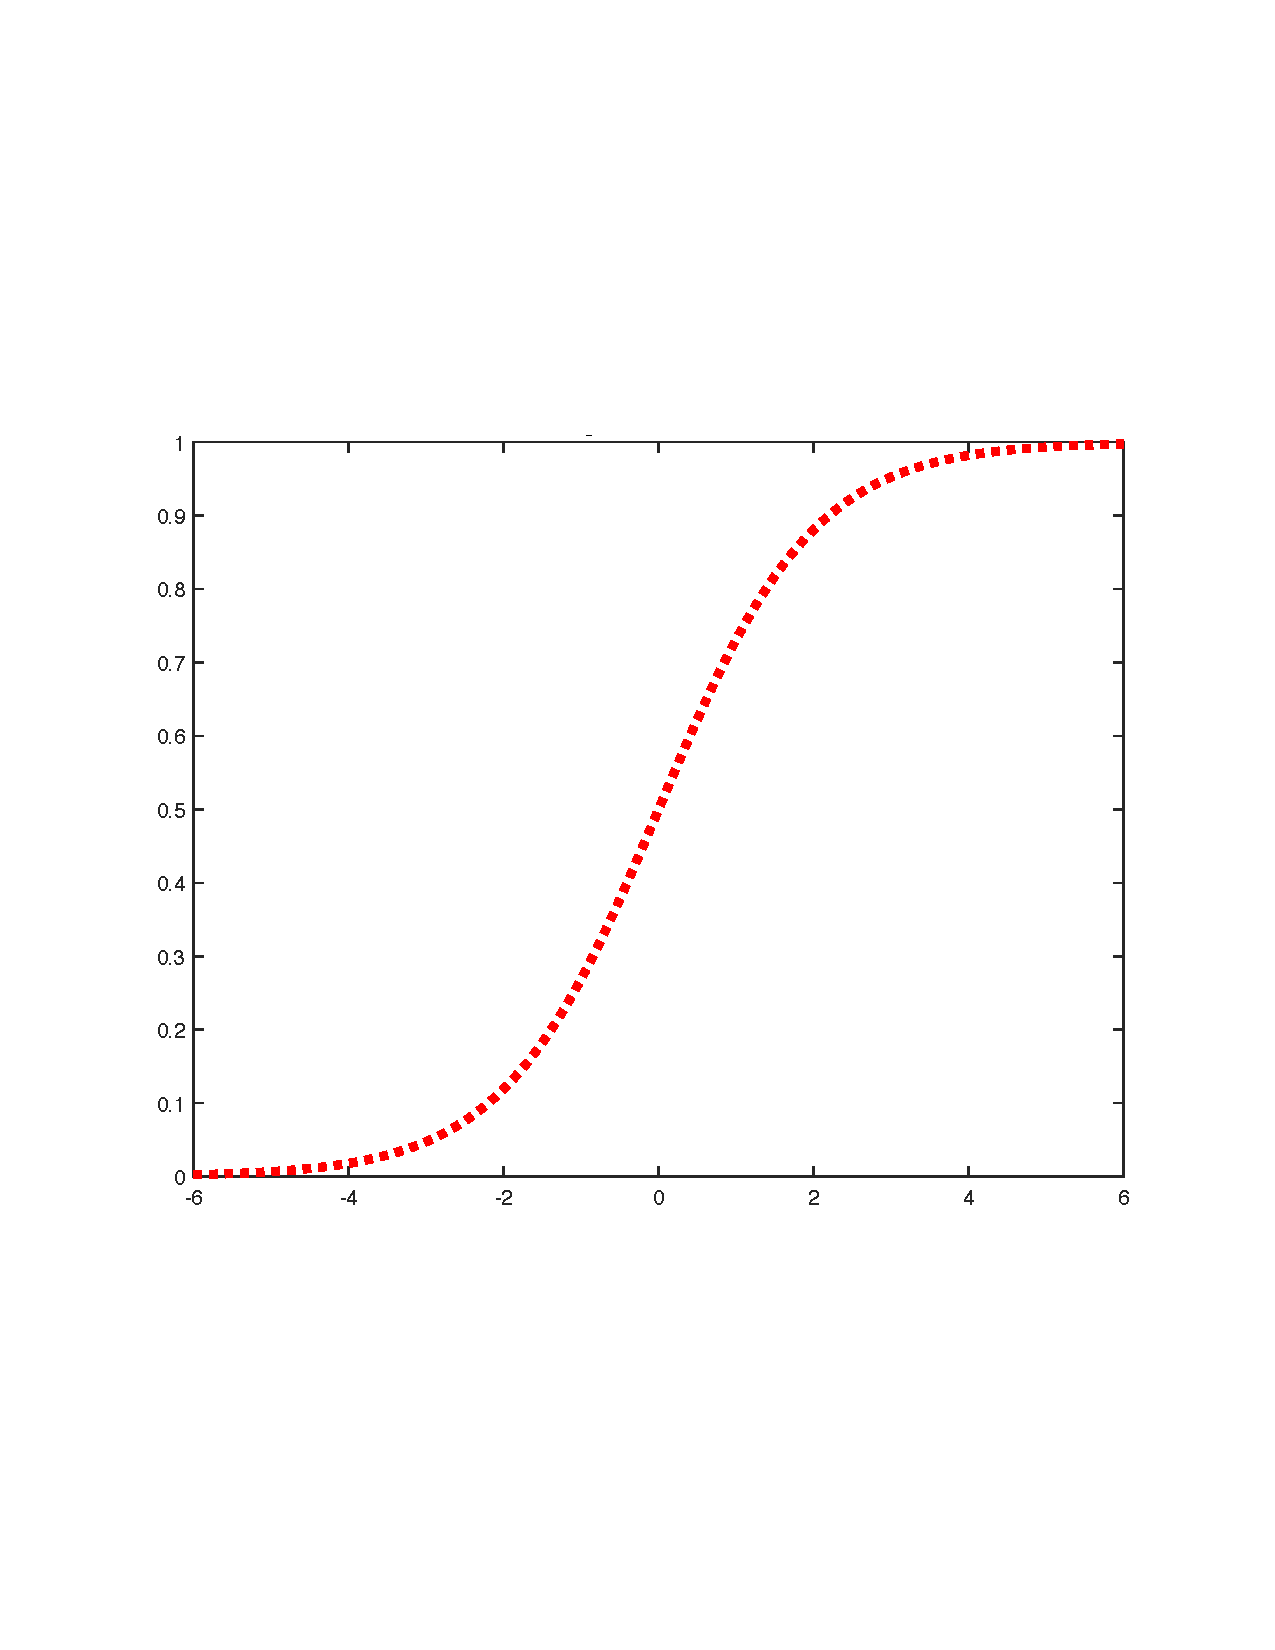
\includegraphics[scale=0.45]{images/SigFunction.pdf}}
\caption{NN activation functions}
\label{marking_image}
\end{center}
\end{figure}

These two functions are very similar in profile, but the \textit{tanh} function is more commonly used due to its favorable back-propagation properties, (i.e. the learning process of the NN). Back-propagation is a key concept in NN and ConvNN, but its description is beyond the scope of this first draft and will most likely be discussed in the final draft of the current document.

\subsection{Logistic Regression Node}

The final layer of the ConvNN is the logistic regression function node, which is a classifier we have reviewed in class. It's functional form is \cite{deep}
\begin{equation}
y_{prediction} \, = \, \text{argmax} P_i (Y = i | \{x, W\})
\end{equation}
where the probability is
\begin{equation}
P_i \, = \, \frac{e^{\vec{w}_i^T \vec{x}_i}}{\sum_j \vec{w}_j^T \vec{x}_j }
\end{equation}
This simply means that the output of the NN is mapped to one of the label of classes, (in this case the level of DR which ranges from 0 to 4).

\subsection{Summary}

So putting all the pieces together,  the ConvNN has the general layout seen in \figref{summary}

\begin{figure}[htbp]
\begin{center}
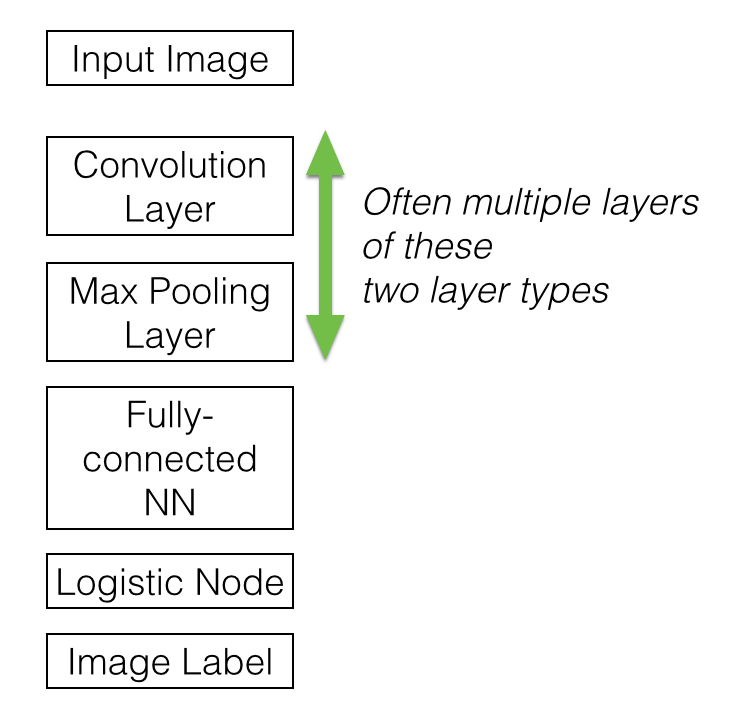
\includegraphics[scale=0.6]{images/summaryNN.png}
\caption{The ConvNN as a whole}
\label{summary}
\end{center}
\end{figure}

As noted in the figure, the convolution layer and the max pooling layer are often stacked multiple times in practice to reduce the overall computational load of the fully connected neural network module, which is often the most computational expensive member of the ConvNN. In the current work, two repetitive blocks of convolution layers and max pooling layers have been used to process the input image.

\section{Current Project Status}

Python is a powerful and flexible language, but it is not entirely ideal to deal with image processing. To manage the challenges of handling such large images in conjunction with the issues related to memory management of Python code, a subsection of the training image data set was used to begin code development. In addition, to assist in dealing with these issues, an instance on EC2, (\textit{Elastic Compute Cloud}), was created to run the code base and train the ConvNN. This work is still ongoing. The currents status update will consist of two parts. The first part will review the code that has been written up to now and the libraries that are being used. The second section will discuss issues relevant to image preparation and the current data set being used. 

\subsection{Code Base}


Initial attempts at writing an entire ConvNN from scratch proved to be too complex for the allotted period of time. To assist in the process, a variety of open-source libraries were imported into the code base to do some of the heavy lifting. To process images, the \textit{openCV} computer vision library was used to load, crop and convert to gray-scale all images in the selected training set. Below is an excerpt from the code that does some of this processing. Once images are loaded and cropped they look as shown in \figref{loaded}.

\begin{verbatim}
 def processD(self):
        # Load left image
        for i in range(0,len(self.lImageNames)):
            print 'Left images being loaded: ' + str(i)
            name = self.imageDPath+self.lImageNames[i]+'.jpeg'
            image = cv2.imread(name,4)
            # crop the image
            image = image[10:2010,610:3010]
            # convert to gray scale
            imageL = cv2.cvtColor(image, cv2.COLOR_BGR2GRAY)
            self.lImageList.append(imageL)
\end{verbatim}

\begin{figure}[htbp]
\begin{center}
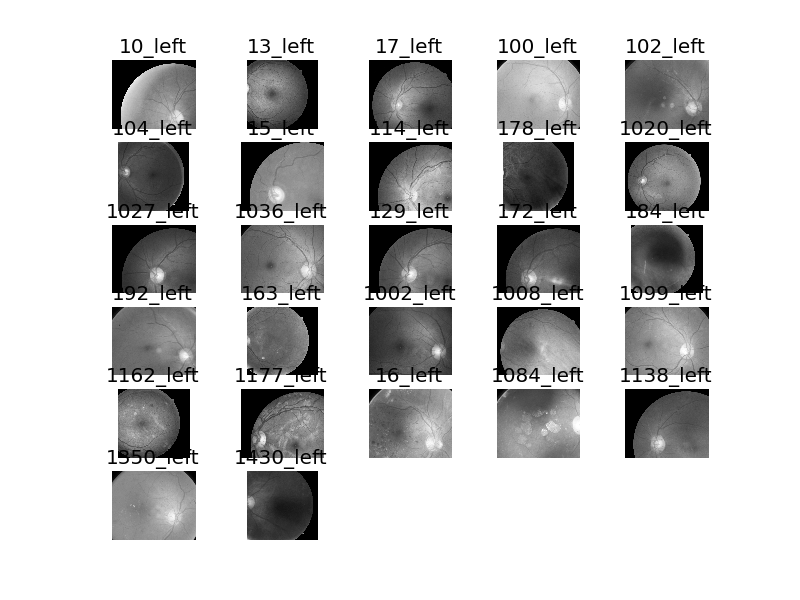
\includegraphics[scale=0.75]{images/lInitialImages_gray.png}
\caption{Images loaded, cropped, and converted to gray-scale}
\label{loaded}
\end{center}
\end{figure}

Manual labels were defined for each of the training, validation and testing data sets.  These data sets consists of the image names and the labels that correspond to them. Data sets are prepared by converting 2D image matrices into 1D row vectors, and then segregating these images into the three distinct groups.

\begin{verbatim}
# Create a database with labels and images
    nPixels = PIXELDIM*PIXELDIM
    dataSetLeft = np.zeros([nImagesSubset,nPixels])
    count = 0 
    for i in range(0,nImagesSubset):
        image = np.reshape(iL.lImageList[i],iL.lImageList[i].shape[0]\
                           *iL.lImageList[i].shape[1],1)
        print i
        dataSetLeft[count,:] = image[0:nPixels]
        count += 1
        
    # Index arrays
    trainIndex = [0,1,2,3,6,7,8,12,13,16,17,18,19,22,23,24]
    validIndex = [4,9,10,14,20,25]
    testIndex = [5,11,15,21,26]
    
    # subset data sets
    trainSetL = prepareData(trainIndex, nPixels, dataSetLeft)
    validSetL = prepareData(validIndex, nPixels, dataSetLeft)
    testSetL = prepareData(testIndex, nPixels, dataSetLeft)
\end{verbatim}
It is noted that the manual index labeling for the different groups is only for code prototyping, and once a more robust code is finished, there will be more random selection for each of these data sets.

To define and train a ConvNN, the deep learning library \textit{theano} was used to create a model. The initial architecture of the ConvNN is two layers of convolution layers, followed by one fully connected NN, with a final logistic regression node to do actual classification of the data. The pertinent sections of code are shown below:

\begin{verbatim}
# First convolution layer
 layer0 = LeNetConvPoolLayer(
        rng,
        input=layer0_input,
        image_shape=(batch_size, 1, nPixels, nPixels),
        filter_shape=(nkerns[0], 1, 15, 15),
        poolsize=(12, 12)
    )
# Second convolution layer
    layer1 = LeNetConvPoolLayer(
        rng,
        input=layer0.output,
        image_shape=(batch_size, nkerns[0], 153, 153),
        filter_shape=(nkerns[1], nkerns[0], 8, 8),
        poolsize=(2, 2)
    )
 # Fully connected layer
     layer2 = HiddenLayer(
        rng,
        input=layer2_input,
        n_in=nkerns[1] * 73 * 73,
        n_out=5,
        activation=T.tanh
    )
   # Classification layer
   layer3 = LogisticRegression(input=layer2.output, n_in=5, n_out=5)
   
  # Entire network 
  params = layer3.params + layer2.params + layer1.params + layer0.params
\end{verbatim}

This concludes the discussion on the current code base. The next section will discuss some elements of the data set preparation.

\subsection{Image Preparation}
\textit{Kaggle} has provided training images in five installments. Filtering through the labels for all training images, we see from \figref{fullSample} that most of the data is heavily skewed toward lower levels of DR, (level 2 and below). To create a more robust training set, equal number of samples of each DR level is being fed to the ConvNN. 

\begin{figure}[htbp]
\begin{center}
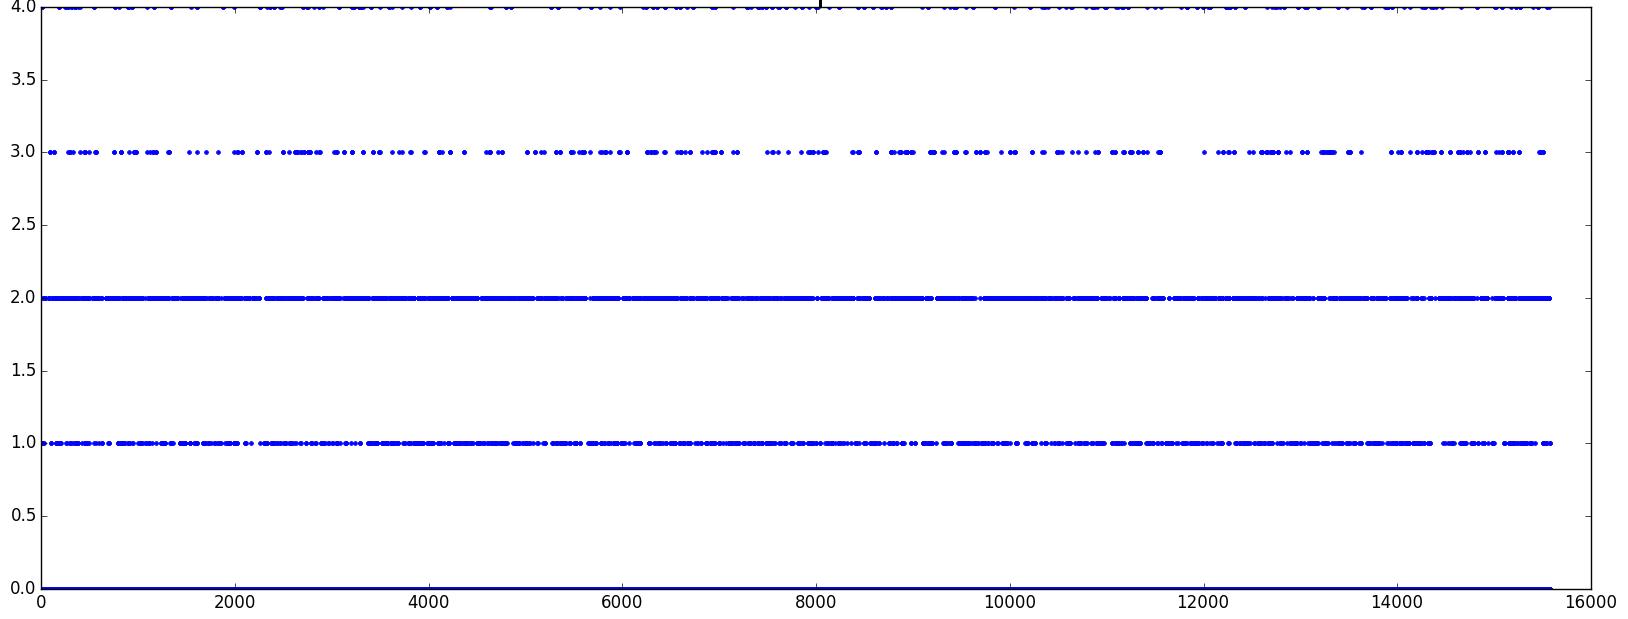
\includegraphics[scale=0.25]{images/FullSample.png}
\caption{All the labels of the training data}
\label{fullSample}
\end{center}
\end{figure}

A code was written to filter the images from the training set, giving the distribution show in \figref{filtered}.

\begin{figure}[htbp]
\begin{center}
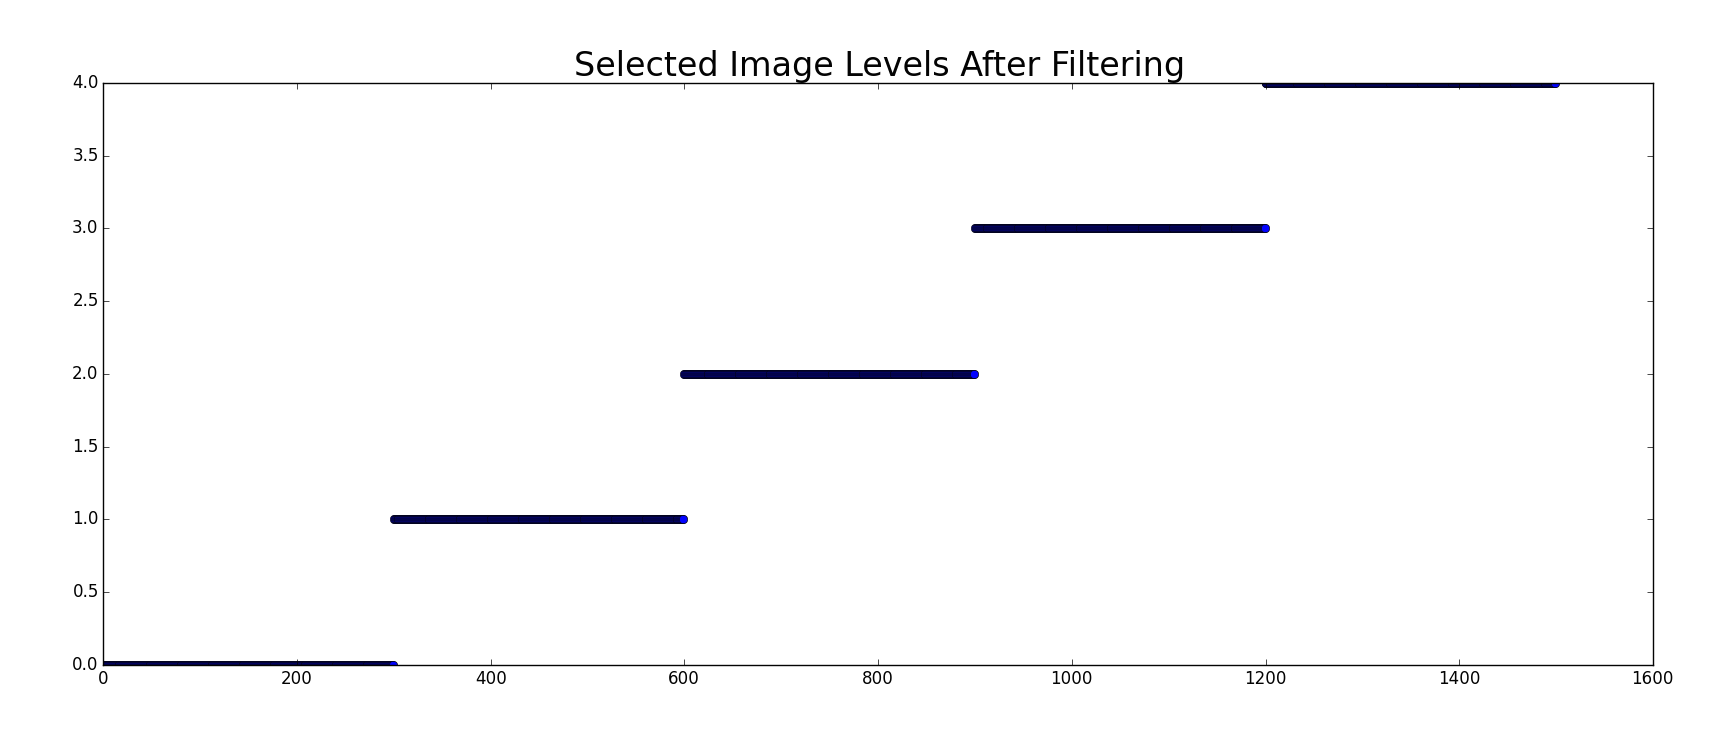
\includegraphics[scale=0.25]{images/After_filtering.png}
\caption{Equal number of DR samples for each category}
\label{filtered}
\end{center}
\end{figure}

For code prototyping, a subset of the images in this filtered data set is being used to train the network.

\section{Conclusion}

Training of the network in ongoing. A variety of challenges still remain, (batch processing on EC2, saving various model files, improving ConvNN architecture, etc.), but hopefully significant strides at bringing the work to reasonable conclusion will be made over the next three weeks. 

% \nocite{*}
\bibliographystyle{unsrt}
\bibliography{References}


\end{document}